\ifx\wholebook\relax \else
% ------------------------

\documentclass[b5paper]{article}
\usepackage[nomarginpar
  %, margin=.5in
]{geometry}

\addtolength{\oddsidemargin}{-0.05in}
\addtolength{\evensidemargin}{-0.05in}
\addtolength{\textwidth}{0.1in}

\usepackage[en]{../../../prelude}

\setcounter{page}{1}

\begin{document}

\title{AVL tree - proofs and the delete algorithm}

\author{Xinyu LIU
\thanks{{\bfseries Xinyu LIU} \newline
  Email: liuxinyu95@gmail.com \newline}
  }

\maketitle
\fi

\markboth{AVL tree - proofs and the delete algorithm}{Elementary Algorithms}

\ifx\wholebook\relax
\chapter{AVL tree - proofs and the delete algorithm}
\numberwithin{Exercise}{chapter}
\fi

\section{Height increment}

When insert an element, the increment of the height can be deduced
into 4 cases:

\be
\begin{array}{rcl}
  \Delta H & = & |T'| - |T| \\
           & = & 1 + max(|r'|, |l'|) - (1 + max(|r|, |l|)) \\
           & = & max(|r'|, |l'|) - max(|r|, |l|) \\
           & = & \begin{cases}
\delta \geq 0, \delta' \geq 0: & \Delta r \\
\delta \leq 0, \delta' \geq 0: & \delta + \Delta r \\
\delta \geq 0, \delta' \leq 0: & \Delta l - \delta \\
otherwise: & \Delta l
\end{cases}
\end{array}
\ee

\begin{proof}
When insert, the height can not increase both on left and right. We can explain the 4 cases from the balance factor definition, that it equals to the difference of the right and left sub-trees:

\begin{itemize}
\item If $\delta \geq 0$ and $\delta' \geq 0$, it means the height
of the right sub-tree is not less than the left sub-tree before and after insertion. In this case, the height increment is only `contributed' from the right, which is $\Delta r$.

\item If $\delta \leq 0$, it means the height of left sub-tree is not less than the right before. Since $\delta' \geq 0$ after insert, we know the height of right sub-tree increases, and the left side keeps same ($|l'|=|l|$). The height increment is:

\[
\begin{array}{rll}
\Delta H & = max(|r'|, |l'|) - max (|r|, |l|) & \{\delta \leq 0\ \text{and}\ \delta' \geq 0 \}\\
         & = |r'|-|l| & \{|l|=|l'|\}\\
         & = |r|+\Delta r - |l| & \\
         & = \delta + \Delta r & \\
\end{array}
\]

\item If $\delta \geq 0$ and $\delta' \leq 0$, similar to the above case, we have the following:

\[
\begin{array}{rll}
\Delta H & = max(|r'|, |l'|) - max (|r|, |l|) & \{\delta \geq 0\ \text{and}\ \delta' \leq 0 \}\\
         & = |l'|-|r| & \\
         & = |l| + \Delta l - |r| & \\
         & = \Delta l - \delta & \\
\end{array}
\]

\item Otherwise, $\delta$ and $\delta'$ are not bigger than zero. It means the height of the left sub-tree is always greater than or equal to the right. The height increment is only `contributed' from the left, which is $\Delta l$.
\end{itemize}
\end{proof}

\section{Balance adjustment after insert}

The balance factors are $\pm 2$ in the 4 cases shown in figure \ref{fig:avl-insert-fix-appendix}. After fixing, $\delta(y)$ resumes
to 0. The height of left and right sub-trees are equal.

\begin{figure}[htbp]
  \centering
  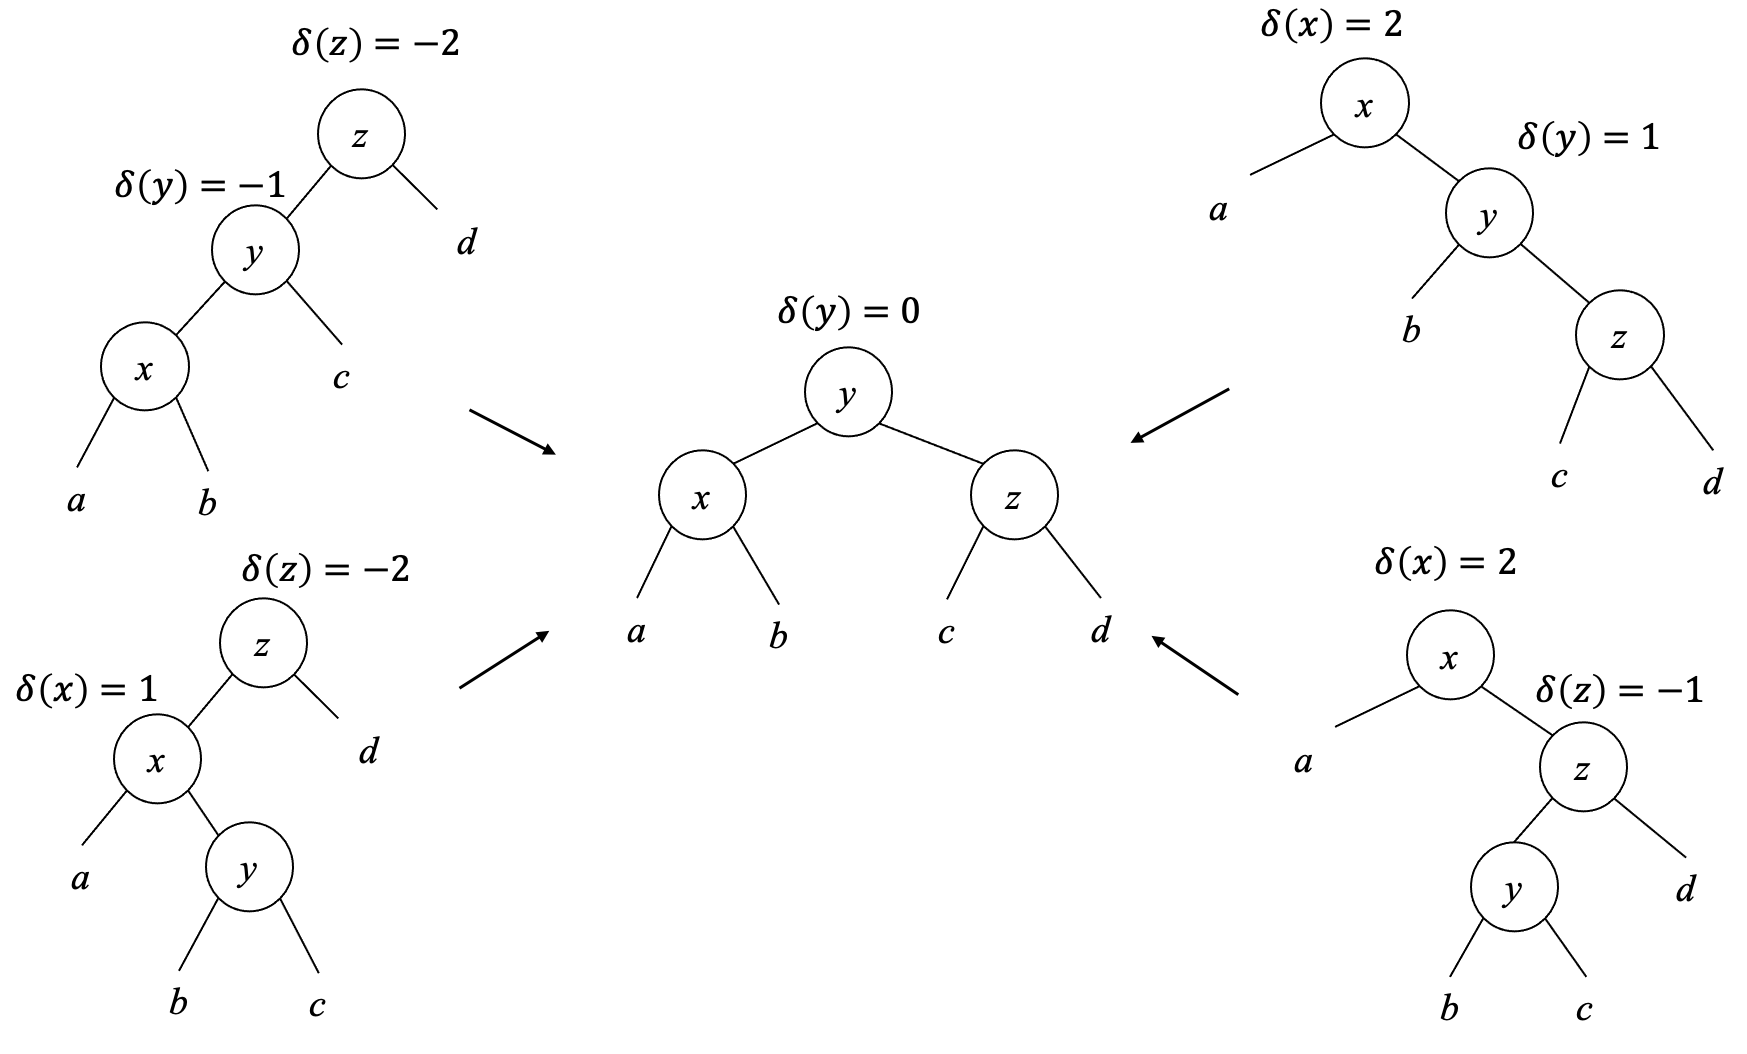
\includegraphics[scale=0.4]{../../../datastruct/tree/AVL-tree/img/avl-insert-fix.png}
  \caption{Fix 4 cases to the same structure}
  \label{fig:avl-insert-fix-appendix}
\end{figure}

The four cases are left-left, right-right, right-left, and left-right. Let the balance factors before fixing be $\delta(x), \delta(y)$, and $\delta(z)$, after fixing, they change to $\delta'(x), \delta'(y)$, and $\delta'(z)$ respectively. We next prove that, $\delta(y)=0$ for all 4 cases after fixing, and give the result of $\delta'(x)$ and $\delta'(z)$.

\subsubsection*{Left-left}

The sub-tree $x$ keeps unchanged, hence $\delta'(x) = \delta(x)$. As $\delta(y) = -1$ and $\delta(z) = -2$, we have:

\be
  \begin{array}{rcl}
  \delta(y) = |c| - |x| = -1 & \Rightarrow & |c| = |x| - 1 \\
  \delta(z) = |d| - |y| = -2 & \Rightarrow & |d| = |y| - 2 \\
  \end{array}
  \label{eq:ll-cd}
\ee

After fixing:

\be
  \begin{array}{rcll}
  \delta'(z) & = & |d| - |c| & \{ from (\ref{eq:ll-cd}) \}\\
             & = & |y| - 2 - (|x| - 1) & \\
             & = & |y| - |x| - 1 & \{  x \text{ is sub-tree of } y \Rightarrow |y|-|x| = 1\} \\
             & = & 0 & \\
  \end{array}
  \label{eq:ll-delta-z}
\ee

For $\delta'(y)$, we have the following:

\be
  \begin{array}{rcll}
  \delta'(y) & = & |z| - |x| & \\
             & = & 1 + max(|c|, |d|) - |x| & \{ \text{by (\ref{eq:ll-delta-z}), } |c| = |d|\} \\
             & = & 1 + |c| - |x| & \{ \text{by (\ref{eq:ll-cd})}\} \\
             & = & 1 + |x| - 1 - |x| & \\
             & = & 0 & \\
  \end{array}
\ee

Summarize the above, the balance factors change to the following in left-left case:

\be
  \begin{array}{l}
  \delta'(x) = \delta(x) \\
  \delta'(y) = 0 \\
  \delta'(z) = 0
  \end{array}
\ee

\subsubsection*{Right-right}

The right-right case is symmetric to left-left:

\be
  \begin{array}{l}
  \delta'(x) = 0 \\
  \delta'(y) = 0 \\
  \delta'(z) = \delta(z)
  \end{array}
  \label{eq:rr-result}
\ee

\subsubsection*{Right-left}

Consider $\delta'(x)$, after fixing, it is:

\be
  \delta'(x) = |b| - |a|
  \label{eq:rl-dx}
\ee

Before fixing, the height of $z$ can be obtained as:

\be
  \begin{array}{rll}
  |z| & = 1 + max(|y|, |d|) &  \{ \delta(z) = -1 \Rightarrow |y| > |d|\} \\
      & = 1 + |y| & \\
      & = 2 + max(|b|, |c|)
  \end{array}
  \label{eq:rl-z}
\ee

Since $\delta(x) = 2$, we have:

\be
  \begin{array}{rll}
  \delta(x) = 2 & \Rightarrow |z| - |a| = 2 & \{ \text{by (\ref{eq:rl-z})} \}\\
                & \Rightarrow 2 + max(|b|, |c|) - |a| = 2 & \\
                & \Rightarrow max(|b|, |c|) - |a| = 0 &
  \end{array}
  \label{eq:rl-ca}
\ee

If $\delta(y) = 1$, then $|c| - |b| = 1$. We have:

\be
  max(|b|, |c|) = |c| = |b| + 1
\ee

Take this into (\ref{eq:rl-ca}) gives:

\be
  \begin{array}{ll}
  |b| + 1 - |a| = 0 \Rightarrow |b|-|a|= -1 & \{ \text{by (\ref{eq:rl-dx}) } \} \\
  \Rightarrow \delta'(x) = -1 &
  \end{array}
\ee

If $\delta(y) \neq 1$, then $max(|b|, |c|) = |b|$. Take this into (\ref{eq:rl-ca}) gives:

\be
  \begin{array}{ll}
  |b| - |a| = 0  & \{ \text{by (\ref{eq:rl-dx})} \} \\
  \Rightarrow \delta'(x) = 0 &
  \end{array}
\ee

Summarize the 2 cases, we obtained the result of $\delta'(x)$ in $\delta(y)$ as the following:

\be
\delta'(x) = \begin{cases}
  \delta(y) = 1: & -1 \\
  otherwise: & 0 \\
\end{cases} \\
\label{eq:rl-dx-dy}
\ee

For $\delta'(z)$, from the definition, it equals to:

\be
  \begin{array}{rcll}
    \delta'(z) & = & |d| - |c| & \{ \delta(z) = -1 = |d| - |y| \} \\
               & = & |y| - |c| - 1 & \{ |y| = 1 + max(|b|, |c|) \} \\
               & = & max(|b|, |c|) - |c| \\
  \end{array}
  \label{eq:rl-dz}
\ee

If $\delta(y) = -1$, then $|c| - |b| = -1$, $max(|b|, |c|) = |b| = |c| + 1$. Take this into (\ref{eq:rl-dz}), we have $\delta'(z) = 1$.

If $\delta(y) \neq -1$, then $max(|b|, |c|) = |c|$. We have $\delta'(z) = 0$.

Combined these two cases, we obtained the result of $\delta'(z)$ in $\delta(y)$ as below:

\be
  \delta'(z) = \begin{cases}
    \delta(y) = -1: & 1 \\
    otherwise: & 0 \\
    \end{cases} \\
  \label{eq:rl-dz-dy}
\ee

Finally, for $\delta'(y)$, we deduce it like below:

\be
  \begin{array}{rl}
  \delta'(y) & = |z| - |x| \\
             & = max(|c|, |d|) - max(|a|, |b|)
  \end{array}
  \label{eq:rl-dy}
\ee

There are three cases:

\begin{itemize}
\item If $\delta(y)=0$, then $|b|=|c|$. According to (\ref{eq:rl-dx-dy}) and (\ref{eq:rl-dz-dy}), we have $\delta'(x)=0 \Rightarrow |a| = |b|$, and $\delta'(z)=0 \Rightarrow |c|=|d|$. These lead to $\delta'(y)=0$.

\item If $\delta(y)=1$, from (\ref{eq:rl-dz-dy}), we have $\delta'(z)=0 \Rightarrow |c| = |d|$.
\[
  \begin{array}{rcll}
  \delta'(y) & = & max(|c|, |d|) - max(|a|, |b|) & \{|c|=|d|\} \\
             & = & |c| - max(|a|, |b|) & \{\text{from (\ref{eq:rl-dx-dy}): $\delta'(x)=-1 \Rightarrow |b|-|a|=-1$} \} \\
             & = & |c| - (|b| + 1) & \{ \delta(y) = 1 \Rightarrow |c|-|b|=1\} \\
             & = & 0 \\
  \end{array}
\]

\item If $\delta(y)=-1$, from (\ref{eq:rl-dx-dy}), we have $\delta'(x)=0 \Rightarrow |a|=|b|$.
\[
  \begin{array}{rcll}
  \delta'(y) & = & max(|c|, |d|) - max(|a|, |b|) & \{|a|=|b|\} \\
             & = & max(|c|, |d|) - |b| & \{ \text{from (\ref{eq:rl-dz-dy}): $|d|-|c|=1$} \} \\
             & = & |c| + 1 - |b| & \{  \delta(y) = -1 \Rightarrow |c|-|b|=-1\} \\
             & = & 0 \\
  \end{array}
\]

\end{itemize}

All three cases lead to the same result $\delta'(y)=0$. Summarize all above, we get the updated balance factors after fixing as below:

\be
  \begin{array}{l}
  \delta'(x) = \begin{cases}
    \delta(y) = 1: & -1 \\
    otherwise: & 0 \\
    \end{cases} \\
  \delta'(y) = 0 \\
  \delta'(z) = \begin{cases}
    \delta(y) = -1: & 1 \\
    otherwise: & 0 \\
    \end{cases} \\
  \end{array}
  \label{eq:rl-result}
\ee

\subsubsection*{Left-right}

Left-right is symmetric to the right-left case. With similar method, we can obtain the new balance factors that is identical to (\ref{eq:rl-result}).

\section{Delete algorithm}

Deletion may reduce the height of the sub-tree. If the balance factor exceeds the range of $[-1, 1]$, then we need fixing.

\subsection{Functional delete}

When delete, we re-use the binary search tree $delete$ in the first step, then check the balance factors and perform fixing. The result is a pair $(T', \Delta H)$, where $T'$ is the new tree and $\Delta H$ is the height decrement. We define $delete$ as below:

\be
delete = \textit{fst} \circ del
\ee

where $del(T, k)$ does the actual work to delete element $k$ from $T$:

\be
\begin{array}{rcl}
del\ \nil\ k & = & (\nil, 0) \\
del\ (l, k', r, \delta) & = & \begin{cases}
  k < k': & tree\ (del\ l\ k)\ k'\ (r, 0)\ \delta \\
  k > k': & tree\ (l, 0)\ k'\ (del\ r\ k)\ \delta \\
  k = k': & \begin{cases}
    l = \nil: & (r, -1) \\
    r = \nil: & (l, -1) \\
    else: & tree\ (l, 0)\ k''\ (del\ r\ k'')\ \delta \\
          & \text{where}\ k'' = min(r) \\
  \end{cases} \\
\end{cases}
\end{array}
\label{eq:avl-del}
\ee

If the tree is empty, the result is $(\nil, 0)$; otherwise, let the tree be $T = (l, k', r, \delta)$. We compare the $k$ and $k'$, lookup and delete recursively. When $k = k'$, we locate the node to be deleted. If it has either empty sub-tree, we cut the node off, and replace it with the other sub-tree; otherwise, we use the minimum $k''$ in the right sub-tree to replace $k'$, and cut $k''$ off. We re-use the $tree$ function and $\Delta H$ result. Additional to the $insert$ cases, there are two cases violate AVL rule, and need fixing. As shown in figure \ref{fig:avl-del-fixing}, both cases can be fixed by a tree rotation. We define them as pattern matching:

\begin{figure}[htbp]
  \centering
  \subcaptionbox{Fix case A}{
    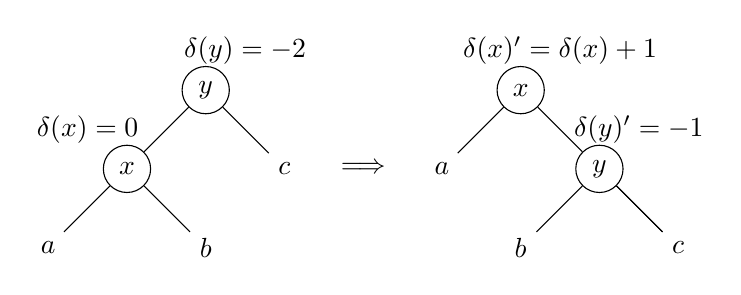
\begin{tikzpicture}[scale=1,
        trnode/.style={circle, draw, inner sep= 0pt, minimum size = .6cm}
      ]
      % left side
      \node[trnode] at (0, 0) (y) {$y$};
      \node[trnode] at (-1, -1) (x) {$x$};
      \draw (1, -1) node (c) {$c$};
      \draw (-2, -2) node (a) {$a$};
      \draw (0, -2) node (b) {$b$};
      % edges
      \draw (y) -- (x) -- (a);
      \draw (y) -- (c);
      \draw (x) -- (b);
      % labels
      \draw (0.5, 0.5) node{$\delta(y) = -2$};
      \draw (-1.5, -0.5) node{$\delta(x) = 0$};

      % right side
      \node[trnode] at (4, 0) (x1) {$x$};
      \draw (3, -1) node (a1) {$a$};
      \node[trnode] at (5, -1) (y1) {$y$};
      \draw (4, -2) node (b1) {$b$};
      \draw (6, -2) node (c1) {$c$};
      % edges
      \draw (x1) -- (y1) -- (c1);
      \draw (x1) -- (a1);
      \draw (y1) -- (b1);
      \draw (y1) -- (c1);
      % labels
      \draw (4.5, 0.5) node{$\delta(x)' = \delta(x) + 1$};
      \draw (5.5, -0.5) node{$\delta(y)' = -1$};

      \draw (2, -1) node{$\Longrightarrow$};
  \end{tikzpicture}} \\
  \subcaptionbox{Fix case B}{
    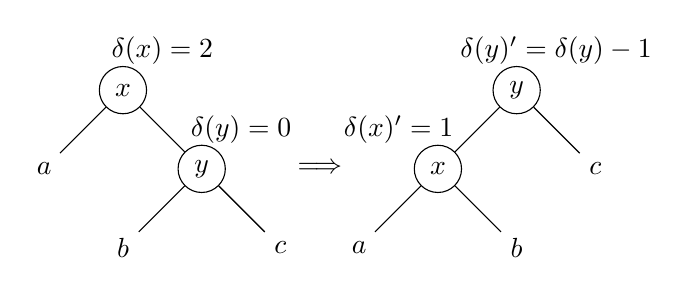
\begin{tikzpicture}[scale=1,
        trnode/.style={circle, draw, inner sep= 0pt, minimum size = .6cm}
      ]
      % left side
      \node[trnode] at (0, 0) (x) {$x$};
      \draw (-1, -1) node (a) {$a$};
      \node[trnode] at (1, -1) (y) {$y$};
      \draw (0, -2) node (b) {$b$};
      \draw (2, -2) node (c) {$c$};
      % edges
      \draw (x) -- (y) -- (c);
      \draw (x) -- (a);
      \draw (y) -- (b);
      \draw (y) -- (c);
      % labels
      \draw (0.5, 0.5) node{$\delta(x) = 2$};
      \draw (1.5, -0.5) node{$\delta(y) = 0$};

      % right side
      \node[trnode] at (5, 0) (y1) {$y$};
      \node[trnode] at (4, -1) (x1) {$x$};
      \draw (6, -1) node (c1) {$c$};
      \draw (3, -2) node (a1) {$a$};
      \draw (5, -2) node (b1) {$b$};
      % edges
      \draw (y1) -- (x1) -- (a1);
      \draw (y1) -- (c1);
      \draw (x1) -- (b1);
      % labels
      \draw (5.5, 0.5) node{$\delta(y)' = \delta(y) - 1$};
      \draw (3.5, -0.5) node{$\delta(x)' = 1$};


      \draw (2.5, -1) node{$\Longrightarrow$};
  \end{tikzpicture}}
  \caption{delete fix}
  \label{fig:avl-del-fixing}
\end{figure}

\be
\begin{array}{rcl}
 ... \\
balance\ ((a, x, b, \delta(x)), y, c, -2)\ \Delta H & = & (a, x, (b, y, c, -1), \delta(x) + 1, \Delta H) \\
balance\ (a, x, (b, y, c, \delta(y)),  2)\ \Delta H & = & ((a, x, b, 1), y, c, \delta(y) - 1, \Delta H) \\
  ... \\
\end{array}
\ee

Below is the example program:

\lstset{frame = single}
\begin{Haskell}
delete t x = fst $ del t x where
  del Empty _ = (Empty, 0)
  del (Br l k r d) x
    | x < k = node (del l x) k (r, 0) d
    | x > k = node (l, 0) k (del r x) d
    | isEmpty l = (r, -1)
    | isEmpty r = (l, -1)
    | otherwise = node (l, 0) k' (del r k') d where k' = min r
\end{Haskell}

Where \texttt{min} and \texttt{isEmpty} are defined as below:

\begin{Haskell}
isEmpty Empty = True
isEmpty _ = False

min (Br Empty x _ _) = x
min (Br l _ _ _) = min l
\end{Haskell}

With the additional two, there are total 7 cases in \texttt{balance} implementation:

\begin{Haskell}
balance (Br (Br (Br a x b dx) y c (-1)) z d (-2), dH) =
        (Br (Br a x b dx) y (Br c z d 0) 0, dH-1)
balance (Br a x (Br b y (Br c z d dz)    1)    2, dH) =
        (Br (Br a x b 0) y (Br c z d dz) 0, dH-1)
balance (Br (Br a x (Br b y c dy)    1) z d (-2), dH) =
        (Br (Br a x b dx') y (Br c z d dz') 0, dH-1) where
    dx' = if dy ==  1 then -1 else 0
    dz' = if dy == -1 then  1 else 0
balance (Br a x (Br (Br b y c dy) z d (-1))    2, dH) =
        (Br (Br a x b dx') y (Br c z d dz') 0, dH-1) where
    dx' = if dy ==  1 then -1 else 0
    dz' = if dy == -1 then  1 else 0
-- Delete specific
balance (Br (Br a x b dx) y c (-2), dH) =
        (Br a x (Br b y c (-1)) (dx+1), dH)
balance (Br a x (Br b y c dy)    2, dH) =
        (Br (Br a x b    1) y c (dy-1), dH)
balance (t, d) = (t, d)
\end{Haskell}

\subsection{Imperative delete}

The imperative $delete$ uses tree rotations for fixing. In the first step, we re-use the binary search tree algorithm to delete the node $x$ from tree $T$; then in the second step, check the balance factor and perform rotation.

\begin{algorithmic}[1]
\Function{Delete}{$T, x$}
  \If{$x = $ NIL}
    \State \Return $T$
  \EndIf
  \State $p \gets$ \Call{Parent}{$x$}
  \If{\Call{Left}{$x$} = NIL}
    \State $y \gets $ \Call{Right}{$x$}
    \State replace $x$ with $y$
  \ElsIf{\Call{Right}{$x$} = NIL}
    \State $y \gets $ \Call{Left}{$x$}
    \State replace $x$ with $y$
  \Else
    \State $z \gets$ \textproc{Min}(\Call{Right}{$x$})
    \State copy data from $z$ to $x$
    \State $p \gets$ \Call{Parent}{$z$}
    \State $y \gets$ \Call{Right}{$z$}
    \State replace $z$ with $y$
  \EndIf
  \State \Return \Call{AVL-Delete-Fix}{$T, p, y$}
\EndFunction
\end{algorithmic}

When delete node $x$, we record its parent in $p$. If either sub-tree is empty, we cut off $x$, and replace it with the other sub-tree. Otherwise if neither sub-tree is empty, we locate the minimum element $z$ of the right sub-tree, copy data from $z$ to $x$, then cut $z$ off. Finally, we call \textproc{AVL-Delete-Fix} with the root $T$, the parent $p$, and the replacement node $y$. Let the balance factor of $p$ be $\delta(p)$, and it changes to $\delta(p)'$ after delete. There are three cases:

\begin{enumerate}
\item $|\delta(p)| = 0$, $|\delta(p)'| = 1$. After delete, although a sub-tree height decreases, the parent still satisfies the AVL
rule. The algorithm terminates as the tree is still balanced;

\item $|\delta(p)| = 1$, $|\delta(p)'| = 0$. Before the delete, the height difference between the two sub-trees is 1; while after delete, the higher sub-tree shrinks by 1. Both sub-trees have the same height now. As the result, the height of the parent also decrease by 1. We need continue the bottom-up update along the parent reference to the root;

\item $|\delta(p)| = 1$, $|\delta(p)'| = 2$. After delete, the tree violates the AVL height rule, we need rotate the tree to fix it.
\end{enumerate}

For case 3, the implementation is similar to the insert fixing. We need add two additional sub-cases as shown in figure \ref{fig:avl-del-fixing}.

\begin{algorithmic}[1]
\Function{AVL-Delete-Fix}{$T, p, x$}
  \While{$p \neq $ NIL}
    \State $l \gets$ \Call{Left}{$p$}, $r \gets$ \Call{Right}{$p$}
    \State $\delta \gets \delta(p)$, $\delta' \gets \delta$
    \If{$x = l$}
      \State $\delta' \gets \delta' + 1$
    \Else
      \State $\delta' \gets \delta' - 1$
    \EndIf
    \If{$p$ is leaf} \Comment{$l = r =$ NIL}
      \State $\delta' \gets 0$
    \EndIf
    \If{$|\delta| = 1 \land |\delta'| = 0$}
      \State $x \gets p$
      \State $p \gets$ \Call{Parent}{$x$}
    \ElsIf{$|\delta| = 0 \land |\delta'| = 1$}
      \State \Return $T$
    \ElsIf{$|\delta| = 1 \land |\delta'| = 2$}
      \If{$\delta' = 2$}
        \If{$\delta(r) = 1$} \Comment{Right-right}
          \State $\delta(p) \gets 0$
          \State $\delta(r) \gets 0$
          \State $p \gets r$
          \State $T \gets $ \Call{Left-Rotate}{$T, p$}
        \ElsIf {$\delta(r) = -1$} \Comment{Right-left}
          \State $\delta_y \gets \delta($ \Call{Left}{$r$} $)$
          \If{$\delta_y = 1$}
            \State $\delta(p) \gets -1$
          \Else
            \State $\delta(p) \gets 0$
          \EndIf
          \State $\delta($ \Call{Left}{$r$} $) \gets 0$
          \If{$\delta_y = -1$}
            \State $\delta(r) \gets 1$
          \Else
            \State $\delta(r) \gets 0$
          \EndIf
        \Else \Comment{Delete specific right-right}
          \State $\delta(p) \gets 1$
          \State $\delta(r) \gets \delta(r) - 1$
          \State $T \gets$ \Call{Left-Rotate}{$T, p$}
          \State break \Comment{No furthur height change}
        \EndIf
      \ElsIf{$\delta' = -2$}
        \If{$\delta(l) = -1$} \Comment{Left-left}
          \State $\delta(p) \gets 0$
          \State $\delta(l) \gets 0$
          \State $p \gets l$
          \State $T \gets $ \Call{Right-Rotate}{$T, p$}
        \ElsIf {$\delta(l) = 1$} \Comment{Left-right}
          \State $\delta_y \gets \delta($ \Call{Right}{$l$} $)$
          \If{$\delta_y = -1$}
            \State $\delta(p) \gets 1$
          \Else
            \State $\delta(p) \gets 0$
          \EndIf
          \State $\delta($ \Call{Right}{$l$} $) \gets 0$
          \If{$\delta_y = 1$}
            \State $\delta(l) \gets -1$
          \Else
            \State $\delta(l) \gets 0$
          \EndIf
        \Else \Comment{Delete specific left-left}
          \State $\delta(p) \gets -1$
          \State $\delta(l) \gets \delta(l) + 1$
          \State $T \gets$ \Call{Right-Rotate}{$T, p$}
          \State break \Comment{No furthur height change}
        \EndIf
      \EndIf
      \Comment{Height decreases, go on bottom-up updating}
      \State $x \gets p$
      \State $p \gets$ \Call{Parent}{$x$}
    \EndIf
  \EndWhile
  \If{$p = $ NIL} \Comment{Delete the root}
    \State \Return $x$
  \EndIf
  \State \Return $T$
\EndFunction
\end{algorithmic}

\begin{Exercise}
\Question{Compare the imperative tree fixing for $insert$ and $delete$, there are similarities. Develop a common fix function for both $insert$ and $delete$.}
\end{Exercise}

\section{Example program}

The main $delete$ program:

\begin{lstlisting}[language = Bourbaki]
Node del(Node t, Node x) {
    if x == null then return t
    Node y
    var parent = x.parent
    if x.left == null {
        y = x.replaceWith(x.right)
    } else if x.right == null {
        y = x.replaceWith(x.left)
    } else {
        y = min(x.right)
        x.key = y.key
        parent = y.parent
        x = y
        y = y.replaceWith(y.right)
    }
    t = deleteFix(t, parent, y)
    release(x)
    return t
}
\end{lstlisting}

Where \texttt{replaceWith} is defined in the chapter of red-black tree. \texttt{release(x)} releases the memory of a node. Function \texttt{deleteFix} is implemented as below:

\begin{lstlisting}[language = Bourbaki]
Node deleteFix(Node t, Node parent, Node x) {
    int d1, d2, dy
    Node p, l, r
    while parent != null {
        d2 = d1 = parent.delta
        d2 = d2 + if x == parent.left then 1 else -1
        if isLeaf(parent) then d2 = 0
        parent.delta = d2
        p = parent
        l = parent.left
        r = parent.right
        if abs(d1) == 1 and abs(d2) == 0 {
            x = parent
            parent = x.parent
        } else if abs(d1) == 0 and abs(d2) == 1 {
            return t
        } else if abs(d1) == 1 and abs(d2) == 2 {
            if d2 == 2 {
                if r.delta == 1 {  // right-right
                    p.delta = 0
                    r.delta = 0
                    parent = r
                    t = leftRotate(t, p)
                } else if r.delta == -1 { // right-left
                    dy = r.left.delta
                    p.delta = if dy == 1 then -1 else 0
                    r.left.delta = 0
                    r.delta = if dy == -1 then 1 else 0
                    parent = r.left
                    t = rightRotate(t, r)
                    t = leftRotate(t, p)
                } else { // delete specific right-right
                    p.delta = 1
                    r.delta = r.delta - 1
                    t = leftRotate(t, p)
                    break // no further height change
                }
            } else if d2 == -2 {
                if (l.delta == -1) { // left-left
                    p.delta = 0
                    l.delta = 0
                    parent = l
                    t = rightRotate(t, p)
                } else if l.delta == 1 { // left-right
                    dy = l.right.delta
                    l.delta = if dy == 1 then -1 else 0
                    l.right.delta = 0
                    p.delta = if dy == -1 then 1 else 0
                    parent = l.right;
                    t = leftRotate(t, l)
                    t = rightRotate(t, p)
                } else { // delete specific left-left
                    p.delta = -1
                    l.delta = l.delta + 1
                    t = rightRotate(t, p)
                    break // no further height change
                }
            }
            // height decreases, go on bottom-up update
            x = parent
            parent = x.parent
        }
    }
    if parent == null then return x // delete the root
    return t
}
\end{lstlisting}

\ifx\wholebook\relax \else
%% \begin{thebibliography}{99}

%% \bibitem{CLRS}
%% Thomas H. Cormen, Charles E. Leiserson, Ronald L. Rivest and Clifford Stein.
%% ``Introduction to Algorithms, Second Edition''. ISBN:0262032937. The MIT Press. 2001

%% \end{thebibliography}

\end{document}
\fi
